\small
\noindent\textbf{$f_r$：Reference selection}\par\smallskip
\begin{minipage}[c]{0.42\textwidth}\centering
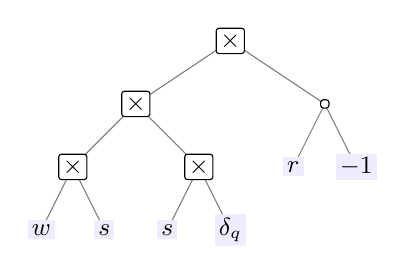
\begin{tikzpicture}[x=8mm,y=8mm,every node/.style={font=\small,inner sep=1.5pt}]
\draw[gray] (0.5,-2) -- (0,-3);
\draw[gray] (0.5,-2) -- (1,-3);
\draw[gray] (2.5,-2) -- (2,-3);
\draw[gray] (2.5,-2) -- (3,-3);
\draw[gray] (1.5,-1) -- (0.5,-2);
\draw[gray] (1.5,-1) -- (2.5,-2);
\draw[gray] (4.5,-1) -- (4,-2);
\draw[gray] (4.5,-1) -- (5,-2);
\draw[gray] (3.0,0) -- (1.5,-1);
\draw[gray] (3.0,0) -- (4.5,-1);
\node[fill=blue!7] at (0,-3) {$w$};
\node[fill=blue!7] at (1,-3) {$s$};
\node[draw,rounded corners=1pt,fill=white] at (0.5,-2) {$\times$};
\node[fill=blue!7] at (2,-3) {$s$};
\node[fill=blue!7] at (3,-3) {$\delta_q$};
\node[draw,rounded corners=1pt,fill=white] at (2.5,-2) {$\times$};
\node[draw,rounded corners=1pt,fill=white] at (1.5,-1) {$\times$};
\node[fill=blue!7] at (4,-2) {$r$};
\node[fill=blue!7] at (5,-2) {$-1$};
\node[draw,rounded corners=1pt,fill=white] at (4.5,-1) {$\AQ$};
\node[draw,rounded corners=1pt,fill=white] at (3.0,0) {$\times$};
\end{tikzpicture}

\end{minipage}\hfill
\begin{minipage}[c]{0.55\textwidth}\small
$w=0.003020$，$s=0.40625$。\par
备选参考路径的相对差距 $\delta_q=0.000000$。\par
\begin{tabular}{@{}lr@{}}\toprule 候选 & Priority score\\\midrule
保留活动路径 & $\mathbf{0.000000}$\\
切换备选路径 & $0.000000$\\
\bottomrule\end{tabular}\par\smallskip
$\Rightarrow r=0$：并列时保留当前参考路径。
\end{minipage}\par\medskip
\noindent\rule{\textwidth}{0.2pt}\par\medskip
\noindent\textbf{$f_j$：Starting-region selection}\par\smallskip
\begin{minipage}[c]{0.42\textwidth}\centering
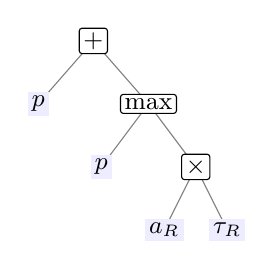
\begin{tikzpicture}[x=8mm,y=8mm,every node/.style={font=\small,inner sep=1.5pt}]
\draw[gray] (2.5,-2) -- (2,-3);
\draw[gray] (2.5,-2) -- (3,-3);
\draw[gray] (1.75,-1) -- (1,-2);
\draw[gray] (1.75,-1) -- (2.5,-2);
\draw[gray] (0.875,0) -- (0,-1);
\draw[gray] (0.875,0) -- (1.75,-1);
\node[fill=blue!7] at (0,-1) {$p$};
\node[fill=blue!7] at (1,-2) {$p$};
\node[fill=blue!7] at (2,-3) {$a_R$};
\node[fill=blue!7] at (3,-3) {$\tau_R$};
\node[draw,rounded corners=1pt,fill=white] at (2.5,-2) {$\times$};
\node[draw,rounded corners=1pt,fill=white] at (1.75,-1) {$\max$};
\node[draw,rounded corners=1pt,fill=white] at (0.875,0) {$+$};
\end{tikzpicture}

\end{minipage}\hfill
\begin{minipage}[c]{0.55\textwidth}\small
$p=0.0198$；各区域$\tau_R\approx 0.99996$。\par
\begin{tabular}{@{}crr@{}}\toprule 区域 & $a_R$ & Priority score\\\midrule
0 & 0.00000 & $0.039600$\\
1 & 0.03125 & $\mathbf{0.051049}$\\
2 & 0.00000 & $0.039600$\\
3 & 0.01562 & $0.039600$\\
\bottomrule\end{tabular}\par\smallskip
$\Rightarrow j=1$：$a_R\tau_R$超过$p$，区域1获得最高分。
\end{minipage}\par\medskip
\noindent\rule{\textwidth}{0.2pt}\par\medskip
\noindent\textbf{$f_k$：Perturbation-intensity selection}\par\smallskip
\begin{minipage}[c]{0.42\textwidth}\centering
\input{generated/structure_conditional_three-s3313_2.tex}
\end{minipage}\hfill
\begin{minipage}[c]{0.55\textwidth}\small
$p=0.0198$，$\rho=0.003964$。\par
\begin{tabular}{@{}crr@{}}\toprule MNE & $u$ & Priority score\\\midrule
2 & 0.25 & $0.273764$\\
4 & 0.50 & $0.523764$\\
8 & 0.75 & $0.773764$\\
16 & 1.00 & $\mathbf{1.023764}$\\
\bottomrule\end{tabular}\par\smallskip
$\Rightarrow\mathrm{MNE}=16$：公共项$p+\rho$不改变$u$的排序。
\end{minipage}\par\medskip
\centering\textbf{最终动作：保留当前参考路径＋区域1＋MNE16}\par
